\let\negmedspace\undefined
\let\negthickspace\undefined
\documentclass[journal]{IEEEtran}
\usepackage[a5paper, margin=10mm, onecolumn]{geometry}
%\usepackage{lmodern} % Ensure lmodern is loaded for pdflatex
\usepackage{tfrupee} % Include tfrupee package

\setlength{\headheight}{1cm} % Set the height of the header box
\setlength{\headsep}{0mm}     % Set the distance between the header box and the top of the text

\usepackage{gvv-book}
\usepackage{gvv}
\usepackage{cite}
\usepackage{amsmath,amssymb,amsfonts,amsthm}
\usepackage{algorithmic}
\usepackage{graphicx}
\usepackage{textcomp}
\usepackage{xcolor}
\usepackage{txfonts}
\usepackage{listings}
\usepackage{enumitem}
\usepackage{mathtools}
\usepackage{gensymb}
\usepackage{comment}
\usepackage[breaklinks=true]{hyperref}
\usepackage{tkz-euclide} 
\usepackage{listings}
% \usepackage{gvv}                               

\def\inputGnumericTable{}                      
\usepackage[latin1]{inputenc}                    
\usepackage{color}                              
\usepackage{array}                             
\usepackage{longtable}                          
\usepackage{calc}                               
\usepackage{multirow}                           
\usepackage{hhline}                            
\usepackage{ifthen}                          
\usepackage{lscape}
\begin{document}

\bibliographystyle{IEEEtran}
\vspace{3cm}

\title{4.4.20}
\author{AI25BTECH11024 - Pratyush Panda
}
\maketitle
% \newpage
% \bigskip
{\let\newpage\relax\maketitle}

\renewcommand{\thefigure}{\theenumi}
\renewcommand{\thetable}{\theenumi}
\setlength{\intextsep}{10pt} % Space between text and floats


\numberwithin{equation}{enumi}
\numberwithin{figure}{enumi}
\renewcommand{\thetable}{\theenumi}

\textbf{Question: } \\
The pair of linear equations $2x=5y+6$ and $15y=6x-18$ represents two lines which are: 
\begin{enumerate}
\item intersecting
\item parallel
\item coincident
\item either intersecting or parallel
\end{enumerate}
\vspace{0.7cm}

\textbf{Solution: } \\
First, let us rewrite the equation of lines as;
\begin{align}
ax+by=c \\
2x-5y=6 \\
6x-15y=18 \textit{ or } 2x-5y=6
\end{align}

Normal vectors of the given lines can be written as:
\begin{align}
\Vec{n}=\myvec{a \\ b} \\
\Vec{n_1}=\myvec{2 \\ -5} && \Vec{n_2}=\myvec{2 \\ -5}
\end{align}

Let the matrix $\Vec{M}$ be;
\begin{align}
\Vec{M}=\myvec{n_1 & n_2}^T=\myvec{2 & -5 \\ 2 & -5}
\end{align}

After reducing it to its Echelon form;
\begin{align}
\myvec{2 & -5 \\ 2 & -5}\xrightarrow{R_2\longleftrightarrow R_2-R_1}\myvec{2 & -5 \\ 0 & 0}
\end{align}

We can see that the rank of $\Vec{M}$ is 1. Therefore, the given lines can be either parallel or coincident.

Now, consider the matrices $\Vec{P}$ and $\Vec{Q}$;
\begin{align}
\Vec{P}=\myvec{a_1 & c_1 \\ a_2 & c_2} && \Vec{Q}=\myvec{b_1 & c_1 \\ b_2 & c_2}
\end{align}
Since, the rank of both the matrices is 1. Thus, we can conclude that the the given lines are coincident.

\begin{figure}[H]
\centering
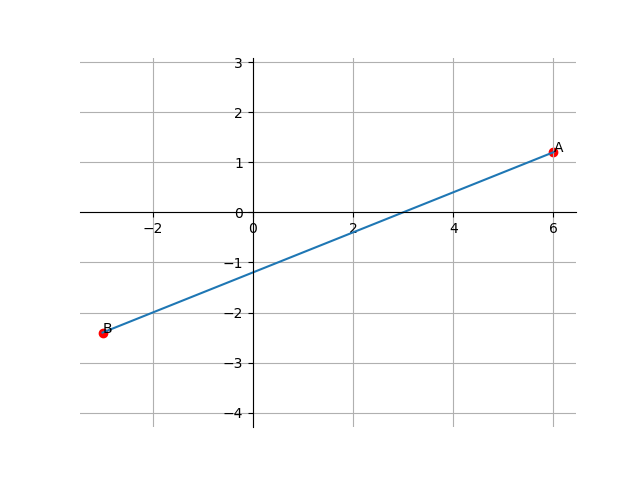
\includegraphics[width=0.8\columnwidth]{figs/img.png}
\caption*{}
\end{figure}

\end{document}